\section{\label{sec:clas.tgt}Hydrogen Target}

The target used by \g12 was a cylindrical liquid hydrogen ($\ell$H$_2$) cell made of Kapton 40~cm in length. The cell was 2~cm in radius while the photon beam had a radial size of approximately 1.5~cm as it \emph{exited} the target. Several experiments prior to \g12 used this same target which could be filled with a number of different materials such as deuterium or helium. The target cell as shown in Fig.~\ref{fig:clas.targetcell} is a simple container design and there is no polarization of the target material.

\begin{figure}\begin{center}
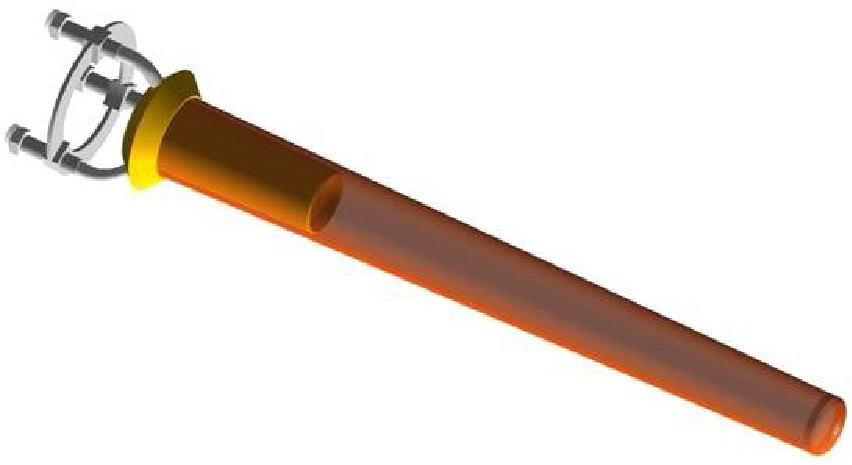
\includegraphics[width=0.6\figwidth]{\grpath/hall-b/g11_target_cell.pdf}
\caption[\g12 Target]{\label{fig:clas.targetcell}The 40~cm long cylindrical Kapton target cell used for \g12.}
\end{center}\end{figure}

\subsection{\label{sec:clas.tgt.position}Position of the Target for \g12}

The typical position of the target for a given experiment with \abbr{CLAS} is at what was called the ``center of \abbr{CLAS}.'' This is a well defined point inside region one of the drift-chambers. With the midpoint of the target cell placed at the center of \abbr{CLAS}, the geometric acceptance begins at about 8$^\circ$ from the beam-line in the lab frame. This configuration optimizes the detection of large angle tracks and is ideal for low energy runs at or below $4$~GeV. As discussed on page~\pageref{sec:clas.hyclas}, the target for \g12 was placed 90~cm upstream of \abbr{CLAS} center which yielded a geometric acceptance starting at approximately 6$^\circ$ from the beam-line. This enabled the optimization of \abbr{CLAS} for small angle track detection.

This placement was not without its drawbacks. Acceptance for large angle tracks was reduced from approximately 140$^\circ$ to 100$^\circ$ in the lab frame, and the drift-chamber resolution was decreased due to the oblique angle the tracks made with the detector planes. The geometric acceptances at large angles decreased in the same way for each subsystem, and the final acceptances in the laboratory frame are shown in the next few sections.
